% Options for packages loaded elsewhere
\PassOptionsToPackage{unicode}{hyperref}
\PassOptionsToPackage{hyphens}{url}
\PassOptionsToPackage{space}{xeCJK}
%
\documentclass[
  ignorenonframetext,
  aspectratio=169,
]{beamer}
\title{プロジェクト全体像：口腔バイオフィルムの群集動態モデリング}
\subtitle{生態 ODE 推定・代謝シミュレーション・空間拡張を束ねる傘}
\author{西岡佳祐 --- NIFE}
\date{2026-06-16}

\usepackage{pgfpages}
\setbeamertemplate{caption}[numbered]
\setbeamertemplate{caption label separator}{: }
\setbeamercolor{caption name}{fg=normal text.fg}
\beamertemplatenavigationsymbolsempty
% Prevent slide breaks in the middle of a paragraph
\widowpenalties 1 10000
\raggedbottom
\setbeamertemplate{part page}{
  \centering
  \begin{beamercolorbox}[sep=16pt,center]{part title}
    \usebeamerfont{part title}\insertpart\par
  \end{beamercolorbox}
}
\setbeamertemplate{section page}{
  \centering
  \begin{beamercolorbox}[sep=12pt,center]{part title}
    \usebeamerfont{section title}\insertsection\par
  \end{beamercolorbox}
}
\setbeamertemplate{subsection page}{
  \centering
  \begin{beamercolorbox}[sep=8pt,center]{part title}
    \usebeamerfont{subsection title}\insertsubsection\par
  \end{beamercolorbox}
}
\AtBeginPart{
  \frame{\partpage}
}
\AtBeginSection{
  \ifbibliography
  \else
    \frame{\sectionpage}
  \fi
}
\AtBeginSubsection{
  \frame{\subsectionpage}
}
\usepackage{amsmath,amssymb}
\usepackage{lmodern}
\usepackage{iftex}
\ifPDFTeX
  \usepackage[T1]{fontenc}
  \usepackage[utf8]{inputenc}
  \usepackage{textcomp} % provide euro and other symbols
\else % if luatex or xetex
  \usepackage{unicode-math}
  \defaultfontfeatures{Scale=MatchLowercase}
  \defaultfontfeatures[\rmfamily]{Ligatures=TeX,Scale=1}
  \setmainfont[]{Noto Serif CJK JP}
  \setmonofont[]{Noto Sans Mono CJK JP}
  \ifXeTeX
    \usepackage{xeCJK}
    \setCJKmainfont[]{Noto Serif CJK JP}
  \fi
  \ifLuaTeX
    \usepackage[]{luatexja-fontspec}
    \setmainjfont[]{Noto Serif CJK JP}
  \fi
\fi
\usetheme[]{Madrid}
\usecolortheme{whale}
\usefonttheme{serif} % use mainfont rather than sansfont for slide text
% Use upquote if available, for straight quotes in verbatim environments
\IfFileExists{upquote.sty}{\usepackage{upquote}}{}
\IfFileExists{microtype.sty}{% use microtype if available
  \usepackage[]{microtype}
  \UseMicrotypeSet[protrusion]{basicmath} % disable protrusion for tt fonts
}{}
\makeatletter
\@ifundefined{KOMAClassName}{% if non-KOMA class
  \IfFileExists{parskip.sty}{%
    \usepackage{parskip}
  }{% else
    \setlength{\parindent}{0pt}
    \setlength{\parskip}{6pt plus 2pt minus 1pt}}
}{% if KOMA class
  \KOMAoptions{parskip=half}}
\makeatother
\usepackage{xcolor}
\IfFileExists{xurl.sty}{\usepackage{xurl}}{} % add URL line breaks if available
\IfFileExists{bookmark.sty}{\usepackage{bookmark}}{\usepackage{hyperref}}
\hypersetup{
  pdftitle={プロジェクト全体像：口腔バイオフィルムの群集動態モデリング},
  pdfauthor={西岡佳祐 --- NIFE},
  hidelinks,
  pdfcreator={LaTeX via pandoc}}
\urlstyle{same} % disable monospaced font for URLs
\newif\ifbibliography
\usepackage{longtable,booktabs,array}
\usepackage{calc} % for calculating minipage widths
\usepackage{caption}
% Make caption package work with longtable
\makeatletter
\def\fnum@table{\tablename~\thetable}
\makeatother
\usepackage{graphicx}
\makeatletter
\def\maxwidth{\ifdim\Gin@nat@width>\linewidth\linewidth\else\Gin@nat@width\fi}
\def\maxheight{\ifdim\Gin@nat@height>\textheight\textheight\else\Gin@nat@height\fi}
\makeatother
% Scale images if necessary, so that they will not overflow the page
% margins by default, and it is still possible to overwrite the defaults
% using explicit options in \includegraphics[width, height, ...]{}
\setkeys{Gin}{width=\maxwidth,height=\maxheight,keepaspectratio}
% Set default figure placement to htbp
\makeatletter
\def\fps@figure{htbp}
\makeatother
\setlength{\emergencystretch}{3em} % prevent overfull lines
\providecommand{\tightlist}{%
  \setlength{\itemsep}{0pt}\setlength{\parskip}{0pt}}
\setcounter{secnumdepth}{-\maxdimen} % remove section numbering
\usepackage{amsmath,amssymb}
\usepackage{tikz}
\usetikzlibrary{arrows.meta,positioning,shapes.geometric,shapes.misc}
\newcommand{\sgn}{\operatorname{sgn}}
\newcommand{\relu}[1]{\left[#1\right]_{+}}
\ifLuaTeX
  \usepackage{selnolig}  % disable illegal ligatures
\fi

\begin{document}
\frame{\titlepage}

\begin{frame}{研究の目的と概要}
\protect\hypertarget{ux7814ux7a76ux306eux76eeux7684ux3068ux6982ux8981}{}
ペリインプラント炎に関わる\textbf{口腔バイオフィルム群集の動態}をモデル化する
（SIIRI コンソーシアム）。

\begin{itemize}
\tightlist
\item
  健常（commensal）から疾患（dysbiotic）への遷移を、群集組成の時間発展として記述する。
\item
  中心的命題：\textbf{ゲノムから計算した代謝が、生態的相互作用の符号を制約する}。
\end{itemize}

\vspace{0.4em}

本デッキは 3 つの緩結合したモデリングの柱と、それらを結ぶ
データ・モデルの共通契約を俯瞰する。
\end{frame}

\begin{frame}{概念図（全体像）}
\protect\hypertarget{ux6982ux5ff5ux56f3ux5168ux4f53ux50cf}{}

\includegraphics[width=\textwidth,height=0.66\textheight]{results/figures/concept_overview_pub.png}

代謝が相互作用の\textbf{符号}を決め、dysbiosis
は\textbf{リワイヤリング＋空間再編}（Pg
の中心化・深部沈降）として現れる。
\end{frame}

\begin{frame}[fragile]{統一オブジェクト --- 10 ギルド分類}
\protect\hypertarget{ux7d71ux4e00ux30aaux30d6ux30b8ux30a7ux30afux30c8-10-ux30aeux30ebux30c9ux5206ux985e}{}
全データ・全モデルが共有する正典 = \textbf{class レベルの 10 ギルド分類}
（\texttt{GUILD\_ORDER}）。

\begin{itemize}
\tightlist
\item
  \texttt{.npy} 配列と JSON
  は、この順序で\textbf{位置インデックス}される。
\item
  各ギルドは代表 AGORA 株を 1 つ持つ（例：Bacilli = \emph{S. gordonii}、
  Negativicutes = \emph{V. parvula}、Bacteroidia = \emph{P.
  melaninogenica}、 Fusobacteriia = \emph{F. nucleatum}）。
\item
  16S 組成 \(\varphi\)、相互作用行列
  \(A\in\mathbb{R}^{10\times10}\)、符号 prior
  \(P\in\{-1,0,+1\}^{10\times10}\) --- すべて同じ 10 軸で揃う。
\end{itemize}

\vspace{0.3em}

この共通分類が、生態・代謝・前処理の 3 つの柱を 1 つの言語で結ぶ。
\end{frame}

\begin{frame}[fragile]{3 つの緩結合モデリングの柱}
\protect\hypertarget{ux3064ux306eux7de9ux7d50ux5408ux30e2ux30c7ux30eaux30f3ux30b0ux306eux67f1}{}
\begin{enumerate}
\tightlist
\item
  \textbf{生態 ODE 推定（論文本体）} --- 縦断 16S から gLV / Hamilton
  相互作用行列を推定。\textbf{代謝符号 prior} で正則化し、
  leave-one-patient-out CV（LOO-CV）で検証。
\item
  \textbf{COMETS / dFBA} ---
  ゲノムスケール（AGORA）の機械論的群集シミュレーション。
  推定された相互作用を独立に交差検証。
\item
  \textbf{16S / メタデータ前処理} --- 生シーケンス + 論文補遺 \(\to\)
  ギルド存在量配列。
\end{enumerate}

\vspace{0.4em}

3 本は独立に走るが、\textbf{10 ギルド分類}と
\textbf{\texttt{fit\_*.json} という交換フォーマット}で接続される。
\end{frame}

\begin{frame}[fragile]{データフロー（実データ）}
\protect\hypertarget{ux30c7ux30fcux30bfux30d5ux30edux30fcux5b9fux30c7ux30fcux30bf}{}

\includegraphics[width=\textwidth,height=0.66\textheight]{results/figures/pipeline_overview_pub.png}

実 Dieckow データ：guild \(\varphi\)（10 患者 \(\times\) 3 週）→ AGORA
符号 prior → gLV/Hamilton フィット（\(\hat A\), \(r=0.95\), SA 70/70）→
LOO-CV 検証 → 4 アトラクター。 \texttt{fit\_*.json} が交換フォーマット。
\end{frame}

\begin{frame}{コアモデル（拡張 Hamilton 原理）}
\protect\hypertarget{ux30b3ux30a2ux30e2ux30c7ux30ebux7c21ux6f54ux7248}{}

\textbf{内部変数}（Klempt et al., 2025）：
$\phi_i\in[0,1]$：体積分率，$\psi_i\in[0,1]$：生存率，
$\bar{\phi}_i:=\phi_i\psi_i$（生存体積分率），$n=5$ 菌種

\textbf{自由エネルギー密度}（栄養濃度 $c^*$ 駆動）：
\[\Psi = -\tfrac{1}{2}c^*\,\bar{\boldsymbol{\phi}}^T\mathbf{A}\,\bar{\boldsymbol{\phi}},
\qquad \mathbf{A}\in\mathbb{R}^{n\times n}\text{（対称成長行列）}\]

$\delta\mathcal{H}=0$ から支配方程式（各菌種 $i$）：
\[0 = -c^*\psi_i\bigl(\mathbf{A}\bar{\boldsymbol{\phi}}\bigr)_i
  + \eta_i\!\left(\dot\phi_i\psi_i^2 + \bar\phi_i\dot\psi_i + \dot\phi_i\right) + \gamma,
\qquad \sum_{l=0}^{n}\phi_l=1\]

\textbf{符号 prior}：AGORA cross-feeding フラックス $F_{ij}$ から
$P_{ij}=\operatorname{sgn}(F_{ij})\in\{-1,0,+1\}$ を作り，
$\mathbf{A}$ の\textbf{符号のみ}を制約（大きさはデータから推定）。
\end{frame}

\begin{frame}{データセット}
\protect\hypertarget{ux30c7ux30fcux30bfux30bbux30c3ux30c8}{}
\begin{longtable}[]{@{}llll@{}}
\toprule
名称 & Accession & 形 & 役割 \\
\midrule
\endhead
Dieckow 2024 & PRJEB71108 & 10 患者 \(\times\) 3 週 & 主要な縦断 fit /
LOO \\
Duran-Pinedo 2021 & PRJNA725874 & 15 患者 \(\times\) 7 時点 &
長期時系列の検証 \\
Szafrański 2025 & mSystems 16S & 127 横断サンプル, 5 属 & アトラクター /
群集型 \\
Heine 2025 & in vitro ODE & --- & 4 つの ODE アトラクター \\
\bottomrule
\end{longtable}

\vspace{0.3em}

Dieckow が一次フィット、Duran-Pinedo が独立コホート、Szafrański
が横断的群集型、 Heine が in vitro の力学的基準を与える。
\end{frame}

\begin{frame}[fragile]{4 つの ODE アトラクター}
\protect\hypertarget{ux3064ux306e-ode-ux30a2ux30c8ux30e9ux30afux30bfux30fc}{}
Heine in vitro 系の 4 状態 = commensal/dysbiotic \(\times\)
static/HOBIC：

\begin{longtable}[]{@{}lll@{}}
\toprule
コード & 群集 & 環境 \\
\midrule
\endhead
\textbf{CS} & commensal & static \\
\textbf{CH} & commensal & HOBIC \\
\textbf{DS} & dysbiotic & static \\
\textbf{DH} & dysbiotic & HOBIC \\
\bottomrule
\end{longtable}

\vspace{0.2em}

\textbf{HOBIC} = チタンインプラント流路チャンバー（flow chamber）。
これらのコードは \texttt{results/} とスクリプト全体で繰り返し現れる。
\end{frame}

\begin{frame}{① 出発点：5 菌種 Bayesian ODE フィット（Heine in-vitro）}
\protect\hypertarget{ux51faux767aux70b95-ux83ccux7a2e-bayesian-ode-ux30d5ux30a3ux30c3ux30c8heine-in-vitro}{}
Heine 2025 の in-vitro 5 菌種（So/An/Vd-Vp/Fn/Pg）時系列に対し ODE
フィットを実施。 \textbf{gLV}（非対称 \(A\)、RMSE 0.012--0.032）と
\textbf{Hamilton NUTS}（対称 \(A\)、RMSE 0.033--0.119） の 2
モデルを比較；4 アトラクター（CS/CH/DS/DH）を再現。


\includegraphics[width=\textwidth,height=0.4\textheight]{results/heine2025/glv_heine_fit_thesis.pdf}

\begin{itemize}
\tightlist
\item
  図：gLV MAP 軌道 + 実験 IQR 箱ひげ図（RMSE は列タイトル）。
\item
  Hamilton NUTS は GPU-TMCMC \(N_p=10{,}000\)；\textbf{独立検証}：pH
  \(R^2=0.78\)、Gingipain--Pg \(r=0.90\)。
\item
  本研究では①を AGORA prior・in-vivo Dieckow・空間
  PDE/FISH（②）へ拡張する。
\end{itemize}
\end{frame}

\begin{frame}{柱 1 --- 相互作用推定と誠実な検証}
\protect\hypertarget{ux67f1-1-ux76f8ux4e92ux4f5cux7528ux63a8ux5b9aux3068ux8aa0ux5b9fux306aux691cux8a3c}{}

\includegraphics[width=\textwidth,height=0.52\textheight]{dieckow_paper/figures/fig2_loo_comparison.png}

\begin{itemize}
\tightlist
\item
  ベストモデルの \textbf{LOO-RMSE \(= 0.0504\)}。
\item
  cross-feeding 方向は独立に検証：\textbf{\(p=4\times10^{-4}\)}。
\item
  2 コホート（Dieckow \(\times\) Duran-Pinedo）が prior 抜きで強ペア符号
  \textbf{89\% 一致}（\(p\approx0.02\)）。
\end{itemize}

\textcolor{red}{prior の価値は予測精度でなく解釈可能性 — 誠実に位置づける。}
\end{frame}

\begin{frame}{柱 1 --- アトラクター構造の検証}
\protect\hypertarget{ux67f1-1-ux30a2ux30c8ux30e9ux30afux30bfux30fcux69cbux9020ux306eux691cux8a3c}{}

\includegraphics[width=\textwidth,height=0.7\textheight]{dieckow_paper/figures/fig3_joshi_attractor.png}

推定した \(A\) から再構成した固定点が、観測された commensal / dysbiotic
群集型に対応する（Joshi アトラクター解析）。動態は単なる回帰ではなく
力学系の構造を持つ。
\end{frame}

\begin{frame}{柱 2 --- COMETS / dFBA}
\protect\hypertarget{ux67f1-2-comets-dfba}{}

\includegraphics[width=\textwidth,height=0.5\textheight]{comets/pipeline_results/sweep_crossfeeding.png}

同じ AGORA GEM が 5 種（So/An/Vp/Fn/Pg）の\textbf{動的
FBA}を前向きに駆動。 フォールバック連鎖：Java COMETS \(\to\)
\textbf{AGORA 較正 Monod dFBA（主経路）} \(\to\) mock
logistic。cross-feeding の\textbf{符号}を構造的に検証（大きさは不問）。
\end{frame}

\begin{frame}[fragile]{柱 3 --- 16S / メタデータ前処理}
\protect\hypertarget{ux67f1-3-16s-ux30e1ux30bfux30c7ux30fcux30bfux524dux51e6ux7406}{}
生シーケンス + 論文補遺から、モデルが消費する\textbf{ギルド \(\varphi\)
配列}を作る：

\begin{itemize}
\tightlist
\item
  \textbf{vsearch + SILVA}（merge \(\to\) QC \(\to\) chimera \(\to\)
  分類）。
\item
  \textbf{QIIME2 / DADA2}、メタゲノムは \textbf{MetaPhlAn}。
\item
  サンプルメタデータは \textbf{Nextflow} パイプライン
  （\texttt{get\_biosample.py} \(\to\) \texttt{merge\_meta.py} \(\to\)
  \texttt{extract\_supp.py}）。
\end{itemize}

\vspace{0.3em}

出力はすべて 10
ギルド分類にマップされ、\(\varphi\;(N_{\text{pat}}\times T\times 10)\)
として柱 1・柱 2 に渡る。
\end{frame}

\begin{frame}{空間拡張（Heine HOBIC FISH）}
\protect\hypertarget{ux7a7aux9593ux62e1ux5f35heine-hobic-fish}{}

\includegraphics[width=\textwidth,height=0.46\textheight]{results/diffusion_fit/zprofiles_all_ti.png}

CLSM-FISH から得た\textbf{深さ分解 5 種プロファイル}を反応拡散方程式で
fit。 dysbiosis は単なる組成変化でなく\textbf{空間的再編成}： \emph{P.
gingivalis} が深部へ沈む（嫌気ニッチ）。0D の gLV を \(z\)
方向の拡散項付き PDE に拡張する。

\medskip
\textbf{限界}：PDE の数値解は収束せず（時間刻み依存・数値不安定）。
図は深さプロファイルの観測量のみ；PDE フィット自体は本体結果から除外し、
補足・今後の課題として扱う。
\end{frame}

\begin{frame}{力学拡張 --- 力学--生物連成の悪循環}
\protect\hypertarget{ux529bux5b66ux62e1ux5f35-ux529bux5b66ux751fux7269ux9023ux6210ux306eux60aaux5faaux74b0}{}

\includegraphics[width=\textwidth,height=0.6\textheight]{masterarbeit_ansys_fem/figures/fem_concept_overview_ja.png}

空間再編（深部 Pg）の力学的帰結：GDI（生物 ODE）→ 炎症 RANKL/OPG →
骨吸収 \(L\) →〔橋渡し \(A(L)\)〕→ 歯槽頂応力 \(\sigma\uparrow\) → RANKL
へ正帰還。柱2（生物）と柱1（力学
FEM）を結ぶ\textbf{悪循環（分岐・双安定）}として患者ごとのリスクを与える。
\end{frame}

\begin{frame}{力学拡張 --- インプラント周囲の応力解析}
\protect\hypertarget{ux529bux5b66ux62e1ux5f35-ux30a4ux30f3ux30d7ux30e9ux30f3ux30c8ux5468ux56f2ux306eux5fdcux529bux89e3ux6790}{}

\includegraphics[width=\textwidth,height=0.64\textheight]{masterarbeit_ansys_fem/figures/fem_implant_crown_section.png}

\begin{enumerate}
[(A)]
\tightlist
\item
  修復インプラントのヘミセクション解剖（crown / gingiva / biofilm / Ti /
  歯 + PDL / 皮質・海綿骨）。(B) 咬合荷重下の \textbf{von Mises 応力
  \(\sigma_{\mathrm{vM}}\)} 断面 ---
  応力は\textbf{歯槽頂（crestal）に集中}し、悪循環の起点となる。
\end{enumerate}
\end{frame}

\begin{frame}[fragile]{サブデッキの接続}
\protect\hypertarget{ux30b5ux30d6ux30c7ux30c3ux30adux306eux63a5ux7d9a}{}
\begin{itemize}
\tightlist
\item
  \textbf{AGORA}（符号 prior）：\(\operatorname{sgn}(F_{ij})\to P_{ij}\)
  を構築する代謝側の橋。
\item
  \textbf{Dieckow（デッキ A）}：その prior 下で \(A\) を推定し LOO
  で検証する本体。
\item
  \textbf{Network（デッキ B）}：推定 \(A\) の構造 --- 中心性・concordant
  backbone・ CS\(\leftrightarrow\)DH リワイヤリングを解析。
\item
  \textbf{Spatial PDE（デッキ C）}：時間動態を深さ方向の反応拡散に拡張。
\item
  \textbf{FISH パイプライン}：CLSM \texttt{.lif} \(\to\)
  深さプロファイル（PDE の観測量）。
\item
  \textbf{Implant FEM（デッキ D）}：組成 \(\to\) 成長固有ひずみ \(\to\)
  界面残留応力 \(\to\) 剥離・歯槽頂応力（力学的読み出し）。
\end{itemize}
\end{frame}

\begin{frame}{現状}
\protect\hypertarget{ux73feux72b6}{}
\begin{longtable}[]{@{}ll@{}}
\toprule
項目 & 状態 \\
\midrule
\endhead
相互作用モデル + 検証 & \textbf{完了}（LOO-RMSE 0.0504,
\(p=4\times10^{-4}\)） \\
空間拡散フィット & \textbf{収束失敗}（数値不安定，限界あり） \\
力学 FEM（剥離・歯槽頂応力） & \textbf{完了}（DH/CH 3.3×, crestal
×1.5） \\
GDI / Joshi 臨床検証 & メタデータ\textbf{待ち} \\
\bottomrule
\end{longtable}

\vspace{0.3em}

2
コホート再現と独立な機械論経路（COMETS）により、相互作用の主張は堅固になりつつある。
空間 PDE は数値不安定により収束せず，本体は ODE + Bayesian 推定 + in-vivo 検証で成立させる。
臨床メタデータ統合は今後の課題。
\end{frame}

\begin{frame}{修士論文の方向性 --- Python 材料モデルの ANSYS 統合}
\protect\hypertarget{masterarbeit-direction}{}

\begin{columns}[T]
\begin{column}{0.52\textwidth}
\textbf{投稿準備中の論文の材料モデル}（Nishioka et al., IKM 2026）\\[4pt]
拡張 Hamilton 原理から導出した自由エネルギー密度：
\[
\Psi = -\tfrac{1}{2}c^*\,\bar{\boldsymbol{\phi}}^{T}\!\mathbf{A}\,\bar{\boldsymbol{\phi}}
\]
$\bar{\phi}_i = \phi_i\psi_i$（生存体積分率），$\mathbf{A}\in\mathbb{R}^{5\times5}$（相互作用行列）\\[4pt]
$\delta\mathcal{H}=0$ から支配方程式（各菌種 $i$）：
\[
0 = -c^*\psi_i(\mathbf{A}\bar{\boldsymbol{\phi}})_i
  + \eta_i\!\left(\dot\phi_i\psi_i^2 + \bar\phi_i\dot\psi_i + \dot\phi_i\right)
  + \gamma
\]
拘束：$\sum_{l=0}^{n}\phi_l = 1$，Newton 法で時間積分
\end{column}
\begin{column}{0.45\textwidth}
\textbf{ANSYS 統合（修士論文）}\\[6pt]
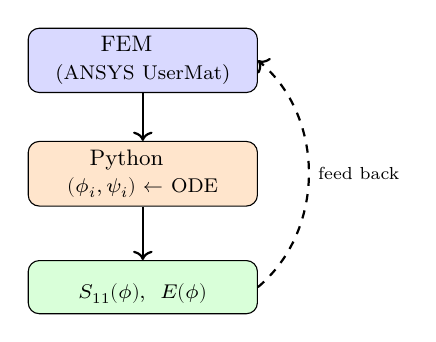
\begin{tikzpicture}[
  boxA/.style={draw,rounded corners,fill=blue!15,text width=3.0cm,align=center,minimum height=0.75cm,font=\small},
  boxB/.style={draw,rounded corners,fill=orange!20,text width=3.0cm,align=center,minimum height=0.75cm,font=\small},
  boxC/.style={draw,rounded corners,fill=green!15,text width=3.0cm,align=center,minimum height=0.75cm,font=\small},
  scale=0.9,transform shape
]
  \node[boxA] (fem) at (0,0)
    {FEM ガウス点\\{\footnotesize (ANSYS UserMat)}};
  \node[boxB] (py) at (0,-1.6)
    {Python 呼び出し\\{\footnotesize $(\phi_i,\psi_i)$ $\leftarrow$ ODE}};
  \node[boxC] (mech) at (0,-3.2)
    {力学特性更新\\{\footnotesize $S_{11}(\phi),\;E(\phi)$}};
  \draw[->,thick] (fem) -- node[right,font=\scriptsize]{現象論モデル置換} (py);
  \draw[->,thick] (py) -- (mech);
  \draw[->,thick,dashed] (mech.east) to[bend right=50]
    node[right,font=\scriptsize]{feed back} (fem.east);
\end{tikzpicture}

\vspace{4pt}
{\footnotesize
指導：第1 Soleimani，第2 Geisler\\
Abaqus フェーズ：2026-05 \textbf{完了} $\checkmark$\\
ANSYS 移植：2026-08〜（次ステップ）}
\end{column}
\end{columns}
\end{frame}

\begin{frame}{Abaqus 実装済み --- プロトタイピングラダー}
\protect\hypertarget{abaqus-ladder}{}

{\small
\begin{tabular}{@{}clll@{}}
\toprule
 & 内容 & 検証結果 & 状態\\
\midrule
1b & Hamilton NSP 単点接線 & 相対誤差 $5\times10^{-5}$ & $\checkmark$\\
2  & Python $\leftrightarrow$ Fortran ソケット & 誤差 0（丸め以下） & $\checkmark$\\
3  & Abaqus UMAT 1要素（小ひずみ） & $\sigma_{xx}=E\varepsilon=50.0$ & $\checkmark$\\
3b & NLGEOM 有限ひずみ成長 & $\lambda_z-1=0.302$，$\sigma_{33}\approx0$ & $\checkmark$\\
3c & 残留応力カラム（深さグレード） & $S_{11}(z)$: $-136\to-354$ MPa & $\checkmark$\\
4  & ANSYS USERMAT & スケルトン（$\texttt{usermat.f}$） & $\cdots$\\
\bottomrule
\end{tabular}
}

\vspace{6pt}
\textbf{Rung 3c の要点}：CLSM 実測 $\phi_{Pg}(z)$ を成長固有ひずみ
$\gamma(z)=\beta\,\phi_{Pg}(z)+c_0$（$\beta=17.2$，$c_0=-1.34$，DH corr $= 0.88$）に変換し，
側面拘束カラム（16 要素）で残留応力分布を計算。\\[4pt]
{\footnotesize
\textbf{未解決}：応力の絶対値は機械測定で未検証（今後の課題）。\\
\textbf{次ステップ}：ANSYS ライセンス取得 $\to$ \texttt{usermat.f} 完成 $\to$ Felix の既存モデルに統合。}
\end{frame}

%% ---------------------------------------------------------------
%%  追加スライド群: Abaqus 実装詳細（村松先生説明用）
%% ---------------------------------------------------------------

\begin{frame}{実装アーキテクチャ --- ガウス点カップリング}
\protect\hypertarget{arch-coupling}{}

\begin{columns}[T]
\begin{column}{0.5\textwidth}
\textbf{FEM Newton ループ内の流れ}\\[4pt]
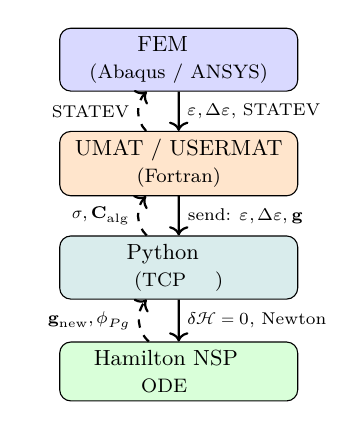
\begin{tikzpicture}[
  bx/.style={draw,rounded corners,fill=gray!10,text width=3.2cm,align=center,
             minimum height=0.65cm,font=\small},
  scale=0.88,transform shape
]
  \node[bx,fill=blue!15] (fem)  at (0, 0)   {FEM ソルバー\\{\footnotesize (Abaqus / ANSYS)}};
  \node[bx,fill=orange!20](umat) at (0,-1.5) {UMAT / USERMAT\\{\footnotesize (Fortran)}};
  \node[bx,fill=teal!15]  (srv)  at (0,-3.0) {Python サーバー\\{\footnotesize (TCP ソケット)}};
  \node[bx,fill=green!15] (nsp)  at (0,-4.5) {Hamilton NSP モデル\\{\footnotesize ODE 時間積分}};
  \draw[->,thick] (fem)  -- node[right,font=\scriptsize]{$\varepsilon,\Delta\varepsilon$, STATEV} (umat);
  \draw[->,thick] (umat) -- node[right,font=\scriptsize]{send: $\varepsilon,\Delta\varepsilon,\mathbf{g}$} (srv);
  \draw[->,thick] (srv)  -- node[right,font=\scriptsize]{$\delta\mathcal{H}=0$, Newton} (nsp);
  \draw[->,thick,dashed] (nsp) to[bend left=45]
    node[left,font=\scriptsize]{$\mathbf{g}_{\rm new},\phi_{Pg}$} (srv);
  \draw[->,thick,dashed] (srv) to[bend left=45]
    node[left,font=\scriptsize]{$\boldsymbol{\sigma}, \mathbf{C}_{\rm alg}$} (umat);
  \draw[->,thick,dashed] (umat) to[bend left=45]
    node[left,font=\scriptsize]{更新 STATEV} (fem);
\end{tikzpicture}
\end{column}
\begin{column}{0.47\textwidth}
\textbf{UMAT インターフェース}\\[4pt]
{\small
\begin{tabular}{@{}ll@{}}
\toprule
Abaqus & 役割\\
\midrule
\texttt{STRAN, DSTRAN} & 全ひずみ + 増分\\
\texttt{STATEV(12)} & NSP 状態 $\mathbf{g}$\\
\texttt{STRESS(6)} & Cauchy 応力（Voigt）\\
\texttt{DDSDDE(6,6)} & 整合接線\\
\bottomrule
\end{tabular}
}\\[8pt]
\textbf{ANSYS USERMAT との対応}\\[2pt]
{\small \texttt{STRESS}$\leftrightarrow$\texttt{stress}，
\texttt{DDSDDE}$\leftrightarrow$\texttt{dsdePl}，
\texttt{STATEV}$\leftrightarrow$\texttt{ustatev}\\
Voigt 順序同一 $\Rightarrow$ Rung 3→4 はほぼコピー}
\end{column}
\end{columns}
\end{frame}

\begin{frame}{Hamilton NSP モデル --- 単点検証（Rung 1b）}
\protect\hypertarget{rung1b-nsp}{}

\begin{columns}[T]
\begin{column}{0.52\textwidth}
\textbf{NSP 状態ベクトル（STATEV）}\\[2pt]
$\mathbf{g} = [\phi_1,\ldots,\phi_5,\;\phi_0,\;\psi_1,\ldots,\psi_5,\;\gamma]^\top \in \mathbb{R}^{12}$\\[4pt]
$\phi_i$：体積分率，$\psi_i$：生存率，$\phi_0$：非生物相，$\gamma$：Lagrange 乗数\\[6pt]

\textbf{1 ステップ更新}（$\delta\mathcal{H}=0$，Newton 法）：
\[
0 = -c^*\psi_i(\mathbf{A}\bar{\boldsymbol\phi})_i
  + \eta_i(\dot\phi_i\psi_i^2 + \bar\phi_i\dot\psi_i + \dot\phi_i) + \gamma
\]
\[
0 = -c^*\phi_i(\mathbf{A}\bar{\boldsymbol\phi})_i
  + \eta_i(\dot\psi_i\phi_i^2 + \bar\phi_i\dot\phi_i)
\]
$\bar\phi_i = \phi_i\psi_i$，拘束 $\sum_{l=0}^{n}\phi_l=1$

\end{column}
\begin{column}{0.45\textwidth}
\textbf{整合接線の検証}\\[4pt]
{\small
\[
\mathbf{C}_{\rm alg} = \frac{\partial \boldsymbol\sigma}{\partial \varepsilon}\bigg|_{\mathbf{g}}
\approx \frac{\boldsymbol\sigma(\varepsilon+h\mathbf{e}_k) - \boldsymbol\sigma(\varepsilon)}{h}
\]
}
各ひずみ経路（$\varepsilon_{11},\varepsilon_{22},\varepsilon_{12}$ 3経路）で
前進差分（$h=10^{-7}$）と照合：

\vspace{4pt}
\begin{center}
\begin{tabular}{@{}lc@{}}
\toprule
チェック & 相対誤差\\
\midrule
Hamilton NSP 接線 & $5\times10^{-5}$ ✓\\
プレースホルダー接線 & $<10^{-11}$ ✓\\
\bottomrule
\end{tabular}
\end{center}

\vspace{4pt}
{\footnotesize
NSP の誤差はヤコビアン行列の AD 精度に由来（JAX \texttt{jacfwd}）；
Newton 収束には十分。}
\end{column}
\end{columns}
\end{frame}

\begin{frame}{成長--力学カップリング（有限ひずみ，Rung 3b）}
\protect\hypertarget{rung3b-fs}{}

\begin{columns}[T]
\begin{column}{0.52\textwidth}
\textbf{乗算的分解}（Bilby--Kröner--Lee）：
\[
\mathbf{F} = \mathbf{F}^e \cdot \mathbf{F}^g
\]
\textbf{成長勾配}（深さ方向のみ膨張）：
\[
\mathbf{F}^g = \mathrm{diag}(1,\;1,\;\lambda_z), \quad
\lambda_z = 1 + \max(0,\,\beta\,\phi_{Pg}(z) + c_0)
\]
CLSM キャリブレーション（DH 系）：
\[
\beta = 17.2,\quad c_0 = -1.34,\quad \text{corr}=0.88
\]
\textbf{弾性部}（compressible neo-Hookean）：
\[
\boldsymbol\sigma = \frac{\mu}{J}(\mathbf{b}^e - \mathbf{I})
  + \frac{\lambda}{J}\ln J\,\mathbf{I}
\]
$\mathbf{b}^e = \mathbf{F}^e(\mathbf{F}^e)^\top$，$J=\det\mathbf{F}^e$

\end{column}
\begin{column}{0.45\textwidth}
\textbf{CLSMキャリブレーション}\\[4pt]

\includegraphics[width=\textwidth]{masterarbeit_ansys_fem/figures/F2_growth_calibration.pdf}
{\footnotesize
HOBIC DH 系の膜厚 $h$ vs $\phi_{Pg}$（CLSM 実測）。\\
$\lambda_z - 1 = \beta\phi_{Pg} + c_0$，$\beta=17.2$，corr $= 0.88$}
\end{column}
\end{columns}
\end{frame}

\begin{frame}{自由膨張・拘束カラム検証（Rung 3, 3b, 3c）}
\protect\hypertarget{rung3c-verify}{}

\begin{columns}[T]
\begin{column}{0.38\textwidth}
\textbf{Rung 3b: 自由膨張（1要素）}\\[4pt]

\includegraphics[width=\textwidth]{masterarbeit_ansys_fem/figures/F3_free_swelling.pdf}
{\footnotesize
$\sigma_{33}=0$（自由端），$U_3^{\rm top} \to 0.302 = \lambda_z-1$ ✓\\
SDV1（NSP ステップカウンタ）：0→20}
\end{column}
\begin{column}{0.58\textwidth}
\textbf{Rung 3c: 残留応力カラム}\\[4pt]

\includegraphics[width=\textwidth]{masterarbeit_ansys_fem/figures/F4_residual_stress_DHvsCH.pdf}
{\footnotesize
16 要素カラム。深さ方向に $\phi_{Pg}(z)$ を CLSM から入力，側面拘束（$u_x=u_y=0$）。\\
\textbf{DH（dysbiotic）}：$S_{11}(z)=-136\cdots-354\,\text{MPa}/\mu$ ，深部高 Pg 域で圧縮大。\\
\textbf{CH（commensal）}：$S_{11}$ 逆符号（Pg 減少 → 収縮）。\\
$S_{33}\approx 0$（自由表面）✓}
\end{column}
\end{columns}
\end{frame}

\begin{frame}{メッシュ収束・検証まとめ（Rung 3c）}
\protect\hypertarget{rung3c-conv}{}

\begin{columns}[T]
\begin{column}{0.45\textwidth}
\textbf{メッシュ収束（$N=4,8,16,32$）}\\[4pt]

\includegraphics[width=\textwidth]{masterarbeit_ansys_fem/figures/F5_mesh_convergence.pdf}
{\footnotesize
ピーク $|S_{11}|$ vs 要素数。$N=16$ で $<1\%$ 差 → 以降 $N=16$ を採用。}
\end{column}
\begin{column}{0.52\textwidth}
\textbf{検証項目まとめ}\\[4pt]
{\small
\begin{tabular}{@{}lll@{}}
\toprule
Rung & 検証量 & 結果\\
\midrule
3  & $\sigma_{xx} = E\varepsilon$ & $50.0$ ✓\\
3b & $U_3^{\rm top} = \lambda_z - 1$ & $0.302$ ✓\\
3b & $\sigma_{33}$（自由端）& $\approx 0$ ✓\\
3b & SDV1 カウンタ & $0\to20$ ✓\\
3c & $S_{11}(z) \propto \phi_{Pg}(z)$ & DH/CH 逆符号 ✓\\
3c & $S_{33}\approx0$ & 自由表面 ✓\\
3c & メッシュ収束 & $N=16$ で $<1\%$ ✓\\
\bottomrule
\end{tabular}
}\\[8pt]
\textbf{未解決（正直な限界）}\\[2pt]
{\small
\begin{itemize}
\item[$\cdot$] $\sigma$ 絶対値の力学的実測との比較なし
\item[$\cdot$] バイオフィルム弾性率 $E$ の不確かさ大（Pa〜kPa 域）
\item[$\cdot$] 双方向カップリング（力学 $\to$ 組成）は今後
\end{itemize}
}
\end{column}
\end{columns}
\end{frame}

\begin{frame}{データ橋渡しと臨床への接続}
\protect\hypertarget{data-bridge}{}

\includegraphics[width=0.92\textwidth,height=0.55\textheight,keepaspectratio]%
  {masterarbeit_ansys_fem/figures/F1b_data_bridge.pdf}

\vspace{4pt}
{\small
\textbf{3 層のデータ橋渡し}（層間の仮定を明示）：
\begin{enumerate}
\item \textbf{患者 16S}（組成 $\phi_i$，深さ情報なし）
  $\xrightarrow{\text{ODE/TMCMC}}$ 相互作用行列 $\mathbf{A}$
\item \textbf{in-vitro HOBIC CLSM}（$\phi_{Pg}(z)$ 深さプロファイル）
  $\xrightarrow{\beta=17.2}$ 成長固有ひずみ $\varepsilon^g(z)$
\item \textbf{Abaqus FEM}（ガウス点カップリング）
  $\to$ 残留応力分布 $S_{11}(z)$ → 剥離リスク
\end{enumerate}
}
\end{frame}

\begin{frame}{次ステップ --- ANSYS 移植と修士論文}
\protect\hypertarget{next-steps}{}

\begin{columns}[T]
\begin{column}{0.5\textwidth}
\textbf{ANSYS 移植（Rung 4）}\\[4pt]
{\small
\begin{tabular}{@{}ll@{}}
\toprule
Abaqus & ANSYS\\
\midrule
\texttt{UMAT} & \texttt{USERMAT}\\
\texttt{STRAN/DSTRAN} & \texttt{eps/deps}\\
\texttt{STRESS(6)} & \texttt{stress(6)}\\
\texttt{DDSDDE(6,6)} & \texttt{dsdePl(6,6)}\\
\texttt{STATEV(12)} & \texttt{ustatev(12)}\\
\bottomrule
\end{tabular}
}\\[6pt]
Voigt 順序・状態変数次元が同一 $\Rightarrow$\\
\texttt{usermat.f} スケルトン → socket 橋渡し追加のみ\\[4pt]
{\footnotesize ブロッカー：ANSYS ライセンス（Geisler 経由で申請中）}
\end{column}
\begin{column}{0.47\textwidth}
\textbf{修士論文 ロードマップ}\\[4pt]
{\small
\begin{tabular}{@{}ll@{}}
\toprule
時期 & マイルストーン\\
\midrule
2026-05 & Abaqus フェーズ完了 ✓\\
2026-08 & ANSYS 移植開始\\
2026-09 & Felix 既存モデルに統合\\
2026-10 & 双方向カップリング試験\\
2026-11 & 発表\\
2026-12 & 提出\\
\bottomrule
\end{tabular}
}\\[8pt]
\textbf{指導体制}\\[2pt]
{\small 第1 Soleimani（Hamilton モデル）\\
第2 Geisler（ANSYS FEM / 既存コード）}
\end{column}
\end{columns}
\end{frame}

%% ---------------------------------------------------------------
%%  コードスニペット + インプラント適用（新実装）
%% ---------------------------------------------------------------

\begin{frame}[fragile]{コード: UMAT ソケット通信（Fortran $\leftrightarrow$ Python）}
\protect\hypertarget{code-umat-socket}{}

\begin{columns}[T]
\begin{column}{0.50\textwidth}
\textbf{Fortran UMAT 送信} (\texttt{umat\_socket\_col.f})\\[2pt]
{\footnotesize\ttfamily
\begin{tabbing}
! ガウス点座標・変形勾配・状態変数を送信\\
write(req, *) NSTATV, \\
\quad\quad COORDS(1), COORDS(2), COORDS(3),  \\
\quad\quad ((DFGRD1(i,j),j=1,3),i=1,3), \\
\quad\quad (STATEV(i),i=1,NSTATV), \\
\quad\quad PROPS(1), PROPS(2)   ! E, nu
\end{tabbing}
\vspace{-4pt}
\begin{tabbing}
! 受信: sigma(6) + C\_alg(36) + statev\_new\\
read(resp) (STRESS(i),i=1,6), \\
\quad\quad  ((DDSDDE(i,j),...)), \\
\quad\quad  (STATEV(i),i=1,NSTATV)
\end{tabbing}
}
\end{column}
\begin{column}{0.47\textwidth}
\textbf{Python サーバー核心} (\texttt{umat\_server\_col.py})\\[2pt]
{\footnotesize\ttfamily
\begin{tabbing}
def handle\_record(tokens):\\
\quad coords = tokens[1:4]   \# COORDS\\
\quad F     = tokens[4:13]   \# DFGRD1\\
\quad statev = tokens[13:14] \# step counter\\
\\
\quad \# 深さ正規化 (CPE4: axis=1, C3D8: 2)\\
\quad z = coords[axis] / height\\
\quad phi\_pg = interp(z, ZPROF)\\
\\
\quad \# F=Fe·Fg → neo-Hookean\\
\quad Fg = diag(1, 1, 1+max(0, beta*phi\_pg+c0))\\
\quad Fe = F @ inv(Fg)\\
\quad sigma = cauchy\_neo\_hookean(Fe)\\
\quad return sigma, C\_alg, step+1
\end{tabbing}
}
\end{column}
\end{columns}
\end{frame}

\begin{frame}[fragile]{インプラントジオメトリへの適用（新規実装）}
\protect\hypertarget{code-implant-umat}{}

\begin{columns}[T]
\begin{column}{0.50\textwidth}
\textbf{旧: 熱膨張アナログ（per-layer）}\\[2pt]
{\footnotesize\ttfamily
\begin{tabbing}
! Nz 層ごとに別材料を定義\\
*MATERIAL, NAME=MAT0   ! z=0層\\
*ELASTIC\\
\quad 5000.0, 0.45\\
*EXPANSION, TYPE=ORTHO\\
\quad 0.0, 0.143, 0.0  ! eps\_yy 固定\\
*MATERIAL, NAME=MAT1   ! z=1層\\
...   \# Nz 個繰り返し
\end{tabbing}
}
\textcolor{red}{\small $\Rightarrow$ NSP 動態なし・β 固定・時間発展なし}
\end{column}
\begin{column}{0.47\textwidth}
\textbf{新: NSP UMAT（\texttt{gen\_implant\_umat\_inp.py}）}\\[2pt]
{\footnotesize\ttfamily
\begin{tabbing}
! 全要素を1材料で統一\\
*SOLID SECTION, ELSET=BIOFILM,\\
\quad MATERIAL=NSP\_BIOFILM\\
*MATERIAL, NAME=NSP\_BIOFILM\\
*USER MATERIAL, CONSTANTS=5\\
\quad 5000.0, 0.45, 17.2, -1.34, 1.0\\
*DEPVAR\\
\quad 1   \# STATEV(1) = ステップ counter
\end{tabbing}
}
\textcolor{teal}{\small $\Rightarrow$ 各ガウス点で COORDS $\to$ Python $\to$ NSP}\\[4pt]
{\footnotesize 実行:}\\
{\footnotesize\ttfamily bash run\_implant\_umat.sh DH thread}
\end{column}
\end{columns}

\vspace{6pt}
\textbf{変更点まとめ}：Nz 個の別材料 → 単一 \texttt{*USER MATERIAL}。
\texttt{--coord-axis 1}（CPE4 の $y$ 座標を深さとして使用）。
NLGEOM=YES で有限ひずみ成長。
\end{frame}

%% ---------------------------------------------------------------
%%  追加スライド群: ここまで
%% ---------------------------------------------------------------


%% ---------------------------------------------------------------
%%  AT2 phase-field × Klempt 変分的整合性（2026-06-29 追記）
%% ---------------------------------------------------------------

\begin{frame}{AT2 phase-field --- Klempt との変分的整合性}
\protect\hypertarget{at2-klempt-variational}{}

\begin{columns}[T]
\begin{column}{0.52\textwidth}
\textbf{なぜ Klempt と相性がよいか：同じ $\Psi_e$ を共有}\\[4pt]
Klempt フレームワーク核心：
\[
\mathbf{F} = \mathbf{F}^e\!\cdot\!\mathbf{F}^v\!\cdot\!\mathbf{F}^g
\;\Rightarrow\; \Psi_e(\mathbf{F}^e)
\]
AT2 損傷エネルギー：
\[
\mathcal{E}[u,d] = \!\int\!
\bigl[(1-d)^2\,\Psi_e
+ \tfrac{G_c}{4\ell}\!\bigl(\tfrac{d^2}{\ell}+\ell|\nabla d|^2\bigr)\bigr]\,dV
\]
AT2 は新しい構成則を\textbf{追加しない} ---
Klempt が計算済みの $\Psi_e$ に劣化関数 $(1-d)^2$ を掛けるだけ。

\vspace{6pt}
\textbf{因果チェーン（一本線）}：
\[
k_{\rm eff}\,t \;\to\; \mathbf{F}^g \;\to\; \mathbf{F}^e
\;\to\; \Psi_e \;\xrightarrow{\Psi_e \ge G_c/(2\ell)}\; d \text{ 核生成}
\]

\end{column}
\begin{column}{0.45\textwidth}
\textbf{CZM との厳密性比較}\\[6pt]
{\small
\begin{tabular}{@{}lll@{}}
\toprule
 & AT2 & CZM \\
\midrule
破壊閾値 & $\Psi_e$（既計算量）& $T=f(\delta)$（別仮定）\\
追加仮定 & $\ell$ のみ & 則全体 \\
変分基盤 & $\partial\mathcal{E}/\partial d=0$ & なし \\
経路指定 & 不要 & 必要 \\
\bottomrule
\end{tabular}
}
\vspace{8pt}

\textbf{新規性}：Klempt 成長力学 $\times$ AT2 $\times$
TMCMC 事後サンプルから $k_{\rm eff}(\phi^*)$ を通じた
破壊時刻予測という縦断的接続は文献未報告。

\vspace{4pt}
{\footnotesize
CZM（界面指定型）は最多使用例だが，
AT2 は $\Psi_e$ 閾値を Klempt と同一変分枠内で定式化できる点で厳密性が高い。}
\end{column}
\end{columns}
\end{frame}

\begin{frame}{AT2 正則化長さ $\ell$ の物理的正当化}
\protect\hypertarget{at2-ell-justify}{}

\begin{columns}[T]
\begin{column}{0.50\textwidth}
\textbf{AT2 cohesive strength 式（Tanné et al.\ 2018）}：
\[
\sigma_c = \sqrt{\frac{3\,E\,G_c}{8\,\ell}}
\]
逆解き：$(E,\,G_c,\,\sigma_c)$ から $\ell$ を決定：
\[
\ell_{\rm phys} = \frac{3\,E\,G_c}{8\,\sigma_c^2}
\]

\textbf{バイオフィルム材料値}：
\begin{itemize}
\item $E = 1000\,\text{Pa}$，
      $G_c = 5\,\text{mJ\,m}^{-2}$（文献）
\item $\sigma_c \approx 500\,\text{Pa}$（口腔 BF 付着強度）
\end{itemize}
\[
\ell_{\rm phys}
= \frac{3\times10^3\times5\times10^{-3}}{8\times(500)^2}
\approx 7.5\,\mu\text{m}
\]
\[
\boxed{\ell_{\rm phys}\approx 5\text{--}8\,\mu\text{m}
\approx \texttt{ELL} = 5\,\mu\text{m} \;\checkmark}
\]

\end{column}
\begin{column}{0.47\textwidth}
\textbf{自己無撞着性まとめ}\\[4pt]
{\small
\begin{tabular}{@{}lcc@{}}
\toprule
$\sigma_c$ [Pa] & $\ell_{\rm phys}$ [$\mu$m] & \texttt{ELL} 整合\\
\midrule
100 & 187 & $\times$ \\
300 & 20.8 & $\triangle$ \\
500 & 7.5 & $\checkmark$ \\
700 & 3.8 & $\checkmark$ \\
\bottomrule
\end{tabular}
}\\[8pt]
$G_c^{\rm lit}=5\,\text{mJ/m}^2$，$\sigma_c\approx500\,\text{Pa}$ で
$\ell=5\,\mu$m は数値的任意パラメータ\textbf{ではない}。\\[6pt]

\textbf{モデル値 $G_c=10^{-5}\,\text{J/m}^2$ の注記}：\\[2pt]
{\small
文献値から 3 桁ずれるが，コア主張
\[
\frac{t_{\rm crit}({\rm DH})}{t_{\rm crit}({\rm CH})}
= k_{\rm ratio} = 2.00
\]
は $G_c$ の絶対値に依存しない
（$G_c$ キャンセル）$\Rightarrow$ 定性結果は堅牢。}
\end{column}
\end{columns}
\end{frame}

\begin{frame}[fragile]{Take-home}
\protect\hypertarget{take-home}{}
\begin{enumerate}
\tightlist
\item
  \textbf{代謝が生態的相互作用の符号を制約する}
  （\(P_{ij}=\operatorname{sgn}(F_{ij})\)；大きさは使わない）。
\item
  dysbiosis は\textbf{リワイヤリング + 空間的再編成}であり、 \emph{P.
  gingivalis} の深部への沈降を伴う。
\item
  その主張は \textbf{2 コホート}（Dieckow \(\times\) Duran-Pinedo, 89\%,
  \(p\approx0.02\)）と \textbf{独立な機械論経路}（COMETS
  dFBA）で再現される。
\item
  すべてを 1 つの \textbf{10 ギルド分類}と \textbf{\texttt{fit\_*.json}}
  が束ねる。
\end{enumerate}
\end{frame}

\end{document}
